\documentclass{article}
\usepackage{listings}
\usepackage{graphicx}
\usepackage[slovene]{babel}
\usepackage{color}
\usepackage{amsmath}
\usepackage[usenames,dvipsnames]{xcolor}
\usepackage[hidelinks]{hyperref}
\usepackage{subcaption}
\usepackage{float}
\usepackage{rotating} 
\usepackage{hyperref}
\usepackage{caption}
\usepackage{siunitx}
\graphicspath{{./images/}}

\setlength{\parindent}{0pt}

\begin{document}

\title{Matematično-fizikalni praktikum \\[3mm] \large Naloga 7}
\author{Luka Papež}
\date{10.\ december 2024}

\begin{center}
    
\includegraphics[width=8cm]{logo-fmf.png}
\end{center}

{
    \let\newpage\relax
    \maketitle
}

\maketitle
\newpage
\section{Naloga}
Čim več metod uporabi za izračun
nihanja matematičnega nihala z začetnim pogojem  $\theta(0)= \theta_0 = 1$,$\dot{\theta}(0)=0$. 
Poišči korak, ki zadošča za natančnost na 3 mesta. Primerjaj
tudi periodično stabilnost shem: pusti, naj teče račun čez 10
ali 20 nihajev in poglej, kako se amplitude nihajev sistematično
kvarijo. Pomagaš si lahko tudi tako, da občasno izračunaš
energijo $E \propto  1-\cos \theta + \frac{\dot{\theta}^2 }{2 \omega_0^2} $. Nariši tudi
ustrezne fazne portrete!.
Z analitično rešitvijo dobimo za nihajni čas $\frac{4}{\omega_0} K\left(\sin^2\frac{\theta_0}{2}\right)$, kjer je $K(m)$ popolni
eliptični integral prve vrste, ki je v SciPy knjižnici in v članku na spletni učilnici podan z:
\[
K(m)=\int\limits_{0}^{1} \frac{d z}{\sqrt{\left(1-z^{2}\right)\left(1-m z^{2}\right)}} = \int\limits_{0}^{\frac{\pi}{2}} \frac{d u}{\sqrt{\left(1-m \sin^2{u}\right)}}
\] 
\section{Uvod}
Gibanje masne točke v polju sil v eni dimenziji opišemo
z diferencialno enačbo drugega reda, z Newtonovim zakonom
\begin{equation*}
m\, \Dd[2]{x}{t} = F \>.
\end{equation*}
Enačba je seveda enakovredna sistemu enačb prvega reda
\[
m\, \Dd{x}{t} = p \;, \qquad \Dd{p}{t} = F
\]
in tako jo tudi rešujemo: kot sistem dveh enačb prvega reda.

Seveda morajo biti na voljo tudi ustrezni začetni pogoji, tipično
$x(t=0)=x_0$ in $dx/dt=v(t=0)=v_0$. Splošnejše gre tu za sistem diferencialnih
enačb drugega reda:
\[
\Dd[n]{y}{x} = f(x,y,y',y'',...),
\]
ki ga lahko prevedemo na sistem enačb prvega reda z uvedbo novih spremenljivk v slogu
gibalne količine pri Netwonovi enačbi ($y'=v,y''=z,...$).

Z nekaj truda se da eksplicitno dokazati, mi pa lahko privzamemo, da so metode za
reševanje enačb hoda (Runge-Kutta 4. reda, prediktor-korektor... ) neposredno uporabne
za reševanje takšnih sistemov enačb in torej aplikabilne v poljubno dimenzijah, kar
naj bi v principu zadovoljilo večino naših zahtev.

Obstaja še posebna kategorija tako imenovanih \emph{simplektičnih} metod, za enačbe, kjer je $f$ le funkcija koordinat, $f(y)$, ki (približno) ohranjajo tudi Hamiltonian,
torej energijo sistema. Najbolj znana metoda je Verlet/St\"ormer/Encke metoda, ki je globalno
natančna do drugega reda in ki točno ohranja tudi vrtilno količino sistema (če je ta v danem problemu smiselna). Rešujemo torej za vsak diskretni korak $n$ velikosti $h$, $x_n=x_0+n \cdot h$:
\[
\Dd[2]{y}{x} = f(y)
\]
in pri diskretizaciji dobimo recept za korak $y_n$ in $v_n=y'_n$:
\begin{eqnarray*}
y_{n+1} &=& y_n + h \cdot v_n + \frac{h^2}{2} \cdot f(y_n) \\
v_{n+1} &=& v_n +  \frac{h}{2} \cdot \left[ f(y_n) + f(y_{n+1}) \right].
\end{eqnarray*}
Alternativno lahko to shemo zapišemo tudi s pomočjo dodatnih vmesnih točk in preskakujemo med lego in hitrostjo z zamikom h/2 (od tod angleško ime 'leapfrog' za ta zapis):
\begin{eqnarray*}
y_{n+1} &=& y_n + h \cdot v_{n+1/2} \\
v_{n+3/2} &=& v_{n+1/2} + h \cdot f(y_{n+1}).
\end{eqnarray*}


V še enem drugačnem zapisu je metoda poznana tudi kot metoda ``Središčne razlike'' (Central Difference Method, CDM), če nas hitrost ne zanima:
\[
y_{n+1} - 2 y_n + y_{n-1} = h^2 \cdot f(y_n),
\]
kjer prvo točko $y_1$ izračunamo po originalni shemi. Metodo CDM lahko uporabljamo tudi
za primere, ko je f tudi funkcija 'časa' x, f(x,y), le da tu simplektičnost ni zagotovljena
(in tudi verjetno ne relevantna).
Za simplektične metode višjih redov je na voljo na primer Forest-Ruth metoda ali Position
Extended Forest-Ruth Like (PEFRL) metoda, ki sta obe globalno četrtega reda in enostavni za
implementacijo.
\newpage
\section{Rešitev}
\subsection{Eulerjeva in RK45 metoda}
Naloga nas postavi pred izziv reševanja diferencialnih enačb v obliki Newtonove enačbe. Torej z drugimi besedami diferencialnimi enačbami drugega reda. Kot glavni primer si poglejmo matematično nihalo. Gibanje opišemo s kotom $\varphi$ kot dimenzijo odmika od ravnovesne lege. Rešujemo torej naslednjo enačbo
\begin{equation}
	\ddot{\varphi} + \frac{g}{l}\sin{\varphi} = 0\text{,}
\end{equation}
kjer $\frac{g}{l}$ predstavlja kvadrat frekvence gibanja $\omega^2$. Za namene našega računanja vzamemo primer $\omega=1$. Za začetek si poglejmo kako se obneseta Eulerjeva metoda in Runge-Kutta-Fehlberg (RK45). 
\begin{figure}[H]
    \centering
    \begin{subfigure}[b]{0.49\textwidth}
		\centering
		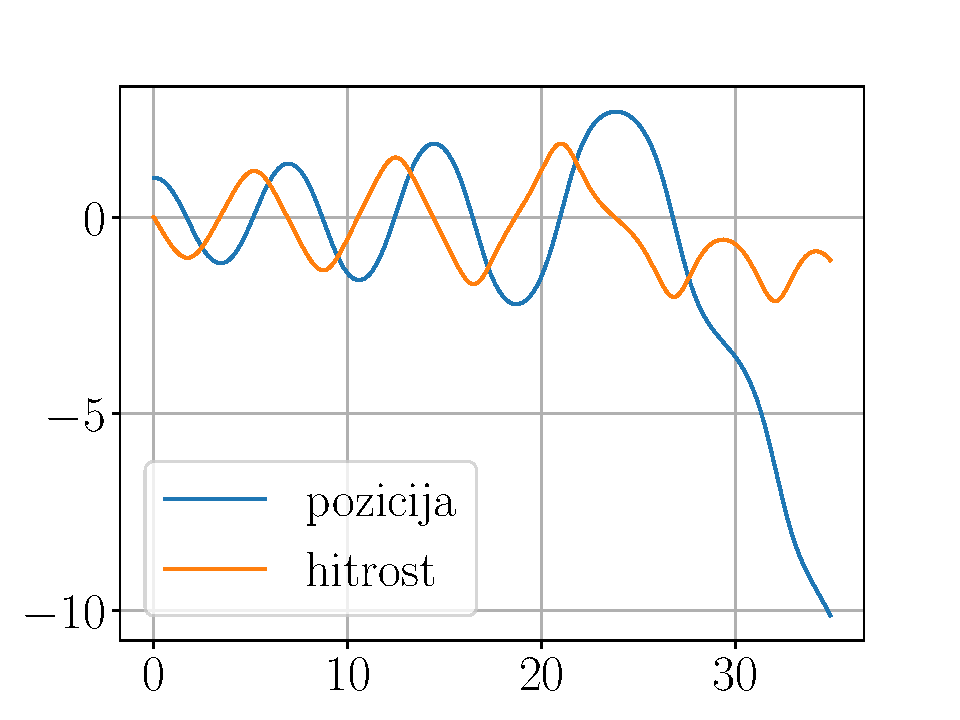
\includegraphics[width=\linewidth]{euler.pdf}
		\caption{Eulerjeva metoda}
    \end{subfigure}
    \hfill
    \begin{subfigure}[b]{0.49\textwidth}
        \centering
        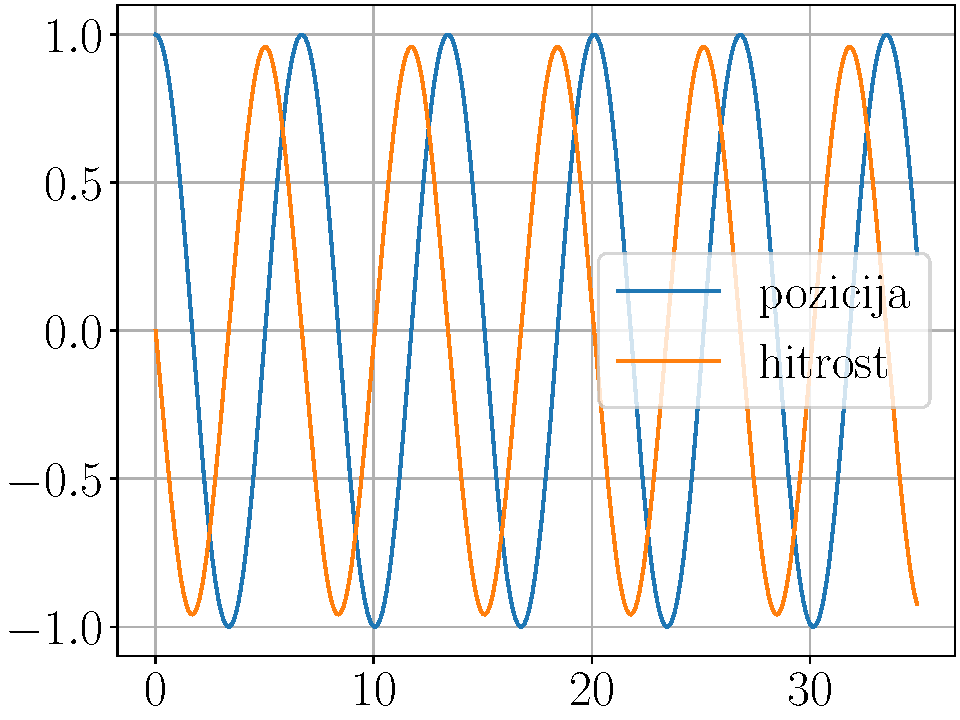
\includegraphics[width=\linewidth]{rk45.pdf}
        \caption{Runge-Kutta 45}
    \end{subfigure}
	\caption{Hitrost in pozicija matematičnega nihala}
\end{figure}
Kot pričakovano po že pridobljenih izkušnjah natančnost Eulerjeve metode na hitrosti precej hitro pridobi velika odstopanja. Posledično pa se izguba natančnosti še toliko bolj opazi pri poziciji. Seveda pa metoda RK45 lepo obdrži natančnost. 

\bigskip

Za ocenjevanje natančnosti so primerne ohranitvene količine. V našem primeru smo izbrali energijo, saj lahko njeno odvisnost $E \propto 1 - \cos{\varphi} + \frac{\dot{\varphi}^2}{2\omega^2}$ enostavno izračunamo z začetnimi pogoji. 
\begin{figure}[H]
	\centering
	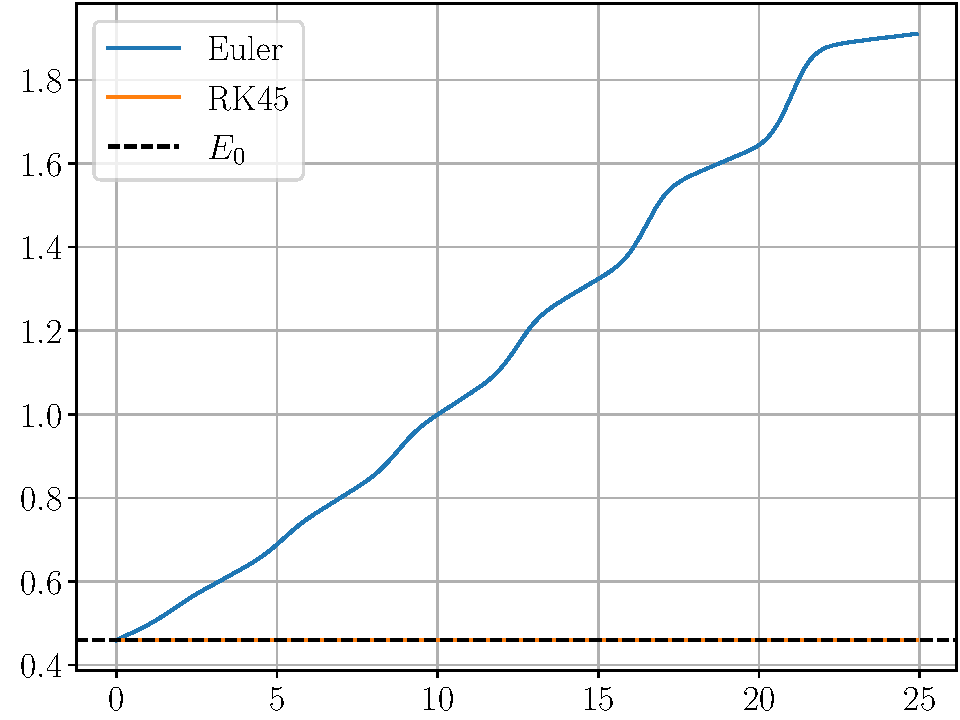
\includegraphics[width=0.7\linewidth]{euler-rk45.pdf}
	\caption{Energija matematičnega nihala pri uporabi Eulerjeve metode in RK45}
\end{figure}
Kot smo razbrali že iz pozicije in hitrosti se očitno energija pri Eulerjevi metodi ne ohranja. Pri metodi RK45 pa je ohranitev precej dobra. 
\subsection{Primerjava različnih metod}
Oglejmo si napake ohranitev energije in potreben čas za izračun pri nekaj reprezentivnih primerih metod integracije.
\begin{figure}[H]
    \centering
    \begin{subfigure}[b]{0.49\textwidth}
		\centering
		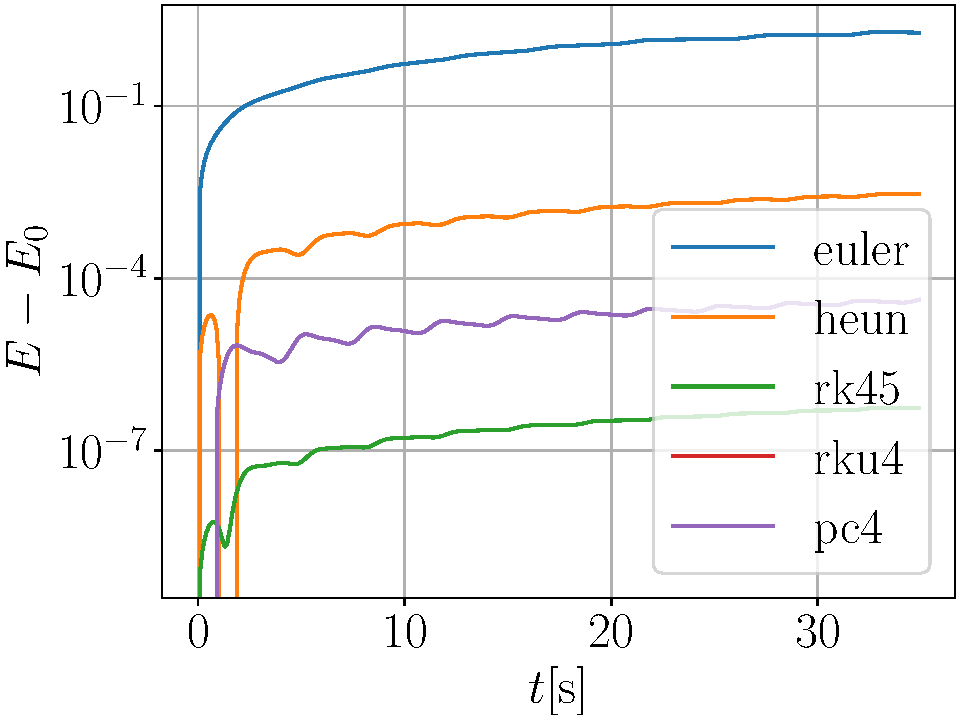
\includegraphics[width=\linewidth]{diffenergy.pdf}
		\caption{Odstopanje od začetne energije}
    \end{subfigure}
    \hfill
    \begin{subfigure}[b]{0.49\textwidth}
        \centering
        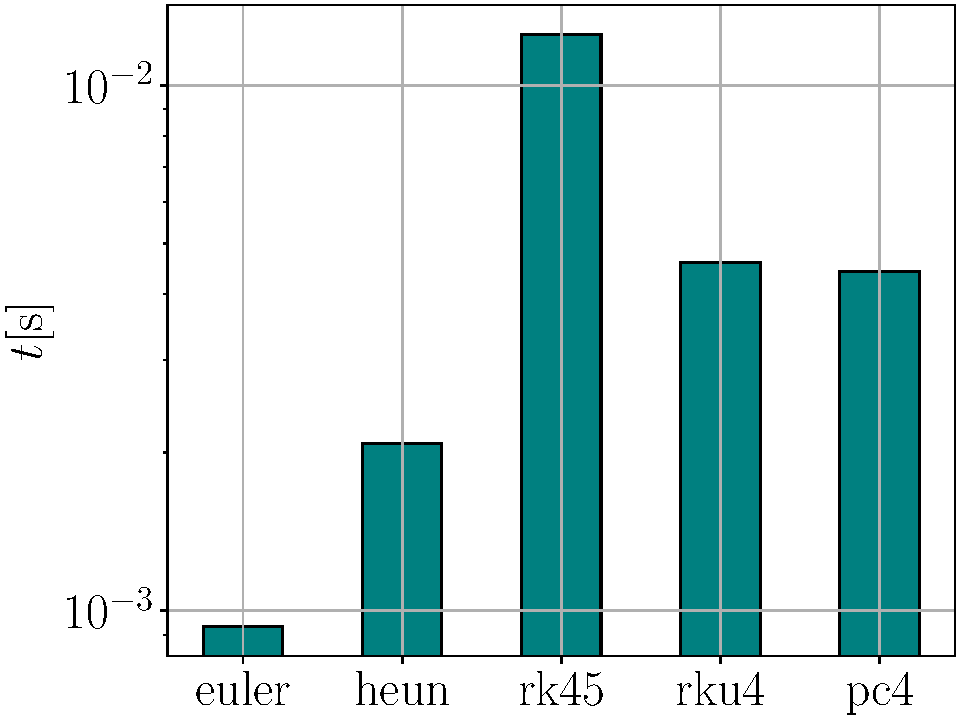
\includegraphics[width=\linewidth]{difftime.pdf}
        \caption{Razlika v računskem času}
    \end{subfigure}
	\caption{Primerjava različnih integracijskih metod}
\end{figure}
Dobimo pričakovane rezultate, kjer je metoda RK45 še najbolj natančna in hkrati najpočasnejša. Poglejmo si še simplektično metodo Leapfrog, ki ohranja stabilnost sistema s pomočjo opravljanja pol korakov. Algoritem je zelo podoben Eulerjevi metodi le, da pozicijo spremenimo s sredinsko vrednostjo hitrosti v intervalu. Poglejmo si kako se energija ohranja v tem primeru.

\begin{figure}[H]
	\centering
	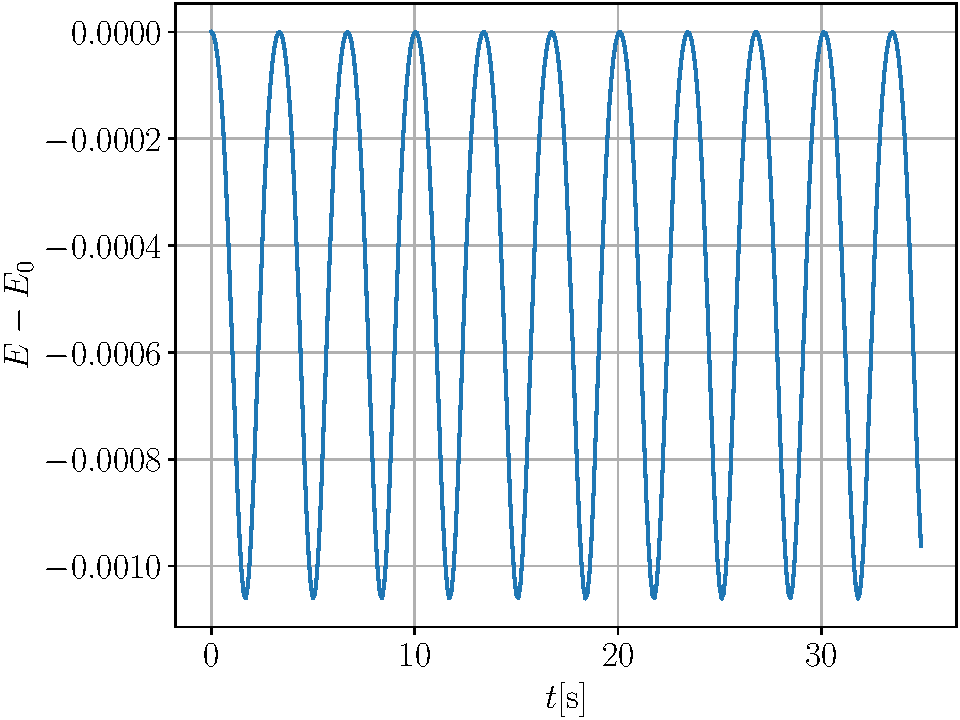
\includegraphics[width=0.7\linewidth]{leapfrog.pdf}
	\caption{Energija matematičnega nihala z uporabo Leapfrog metode}
\end{figure}
Dobimo zanimiv rezultat. Za razliko od ostalih metod, kjer napaka relativno konsistentno narašča, energija tu oscilira pod pravo vrednostjo energije. Najvišja napaka je sicer bližje manj natančnim metodam, a bi to lahko izboljšali z zmanjšanjem koraka. Časovno pa je metoda z $\SI{1.2}{\milli\second}$ primerljiva s hitrostjo Eulerjeve metode.
\subsection{Fazni prostor}
Za konec pa narišemo še fazni prostor. Na našem grafu vsaka posamezna krivulja predstavlja pot matematičnega nihala z začetno pozicijo $\varphi=0$ in določeno začetno hitrost glede na pozicijo na grafu. Da so naše krivulje čim bolj sklenjene pa si pomagamo z izračunom nihajnega časa. To storimo z analitično rešitvijo $\frac{4}{\omega}K\left(\sin^2{\frac{\varphi_0}{2}}\right)$, kjer je $K(m)$ popolni eliptični integral prve vrste, $\varphi_0$ amplituda in $\omega$ frekvenca nihala.
\begin{equation*}
	K(m) = \int_0^{\frac{\pi}{2}}\frac{du}{\sqrt{1 - m\sin^2{u}}}
\end{equation*}

\begin{figure}[H]
	\centering
	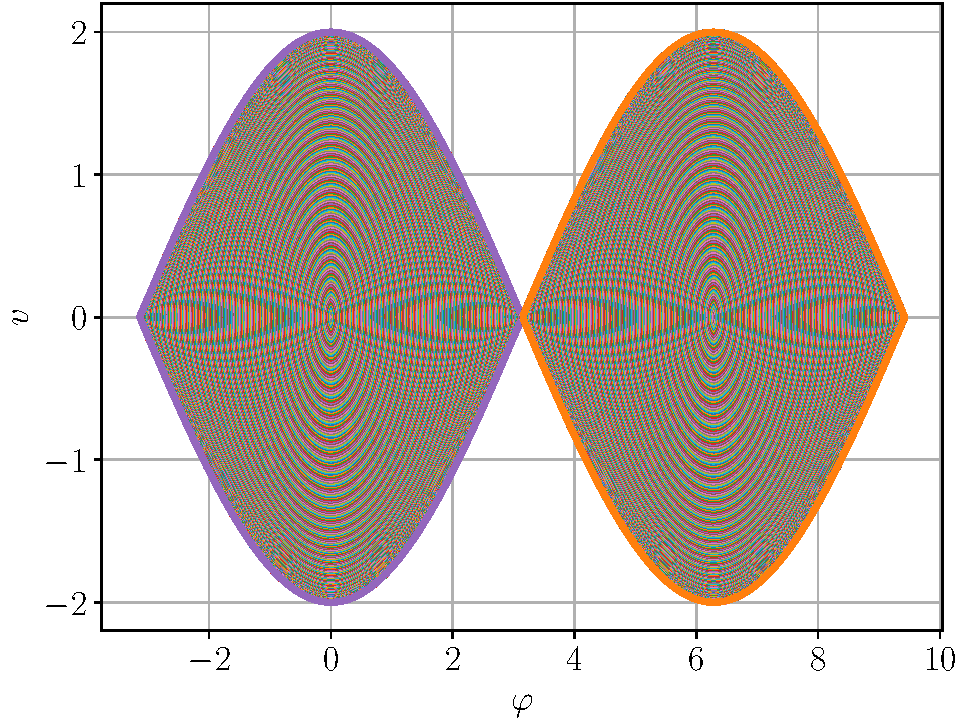
\includegraphics[width=0.7\linewidth]{phase.pdf}
	\caption{Fazni prostor matematičnega nihala}
\end{figure}
Pri manjših amplitudah so poti elipse, ko se amplituda povečuje pa se vedno bolj približuje nezveznosti. Največji odmik nato opazimo pri vrednosti $\pi$(zaradi izbrane frekvence $\omega=1$) čez katero se graf zrcali. Če bi še naprej risali z večjim odmikom $\varphi$ bi se tako na vrednostih $2k\pi - \pi$ ponovil zgornji vzorec. 
\section{Zaključek}
Tokratna naloga je bila podobna prejšnji le, da smo povečali red diferencialne enačbe. Na žalost mi sicer ni uspelo najti časa, da bi rešil tudi dodatne naloge, ki so izgledale kar precej zanimive. 
\href{https://adventofcode.com/2024}{Sem pa zato namenil nekaj več časa vsako letnemu reševanju božiča. Letos je namreč izginil glavni zgodovinar, ki je vedno prisoten pri odhodu božičkovih sank}.

\end{document}
